\begin{savequote}[8cm]
\textlatin{Neque porro quisquam est qui dolorem ipsum quia dolor sit amet, consectetur, adipisci velit...}

There is no one who loves pain itself, who seeks after it and wants to have it, simply because it is pain...
  \qauthor{--- Cicero's \textit{de Finibus Bonorum et Malorum}}
\end{savequote}

\chapter{\label{ch:t2k}The T2K Experiment} 

\minitoc
The T2K experiment is a long-baseline neutrino experiment, aiming to measure CP violation in the lepton sector through neutrino oscillation measurements.
This chapter will first describe the experimental setup and provide a brief overview of the software, which forms the foundation for understanding and discussing the subsequent analyses.


\section{Hardware}
As a long-baseline experiment, T2K comprises a near detector, ND280, and a far detector, Super-Kamiokande (Super-K).
To measure neutrino oscillation, both detectors need to discriminate between \(\numu\) and \(\nue\).  
Of course, no detector can detect neutrinos directly.
In practice, both detectors should possess the capability to distinguish the different products arising from neutrino interactions with the detector’s active material.
The most common products of neutrino–nucleus interactions are the corresponding leptons (i.e.\ electrons and muons) and several hadrons, including protons, neutrons, and light mesons like pions.

The far detector, SK, is a large water Cherenkov detector.
It detects particles by capturing the Cherenkov light emitted when they travel faster than the speed of light in water.
Hadrons produced in neutrino interactions are typically not energetic enough to emit Cherenkov radiation, whereas leptons often travel fast enough.
Hence, SK primarily measures electrons and muons.
The Cherenkov radiation from these leptons typically forms ring-like patterns perpendicular to their direction of motion.
Due to the lighter mass of the electron, its propagation is more susceptible to scattering, making its Cherenkov ring more diffuse compared to the muon’s, as shown in Fig.~\ref{fig:sk-e-mu}.

\begin{figure}
    \centering
    \begin{subfigure}[b]{\dbfigwid\textwidth}
        \centering
        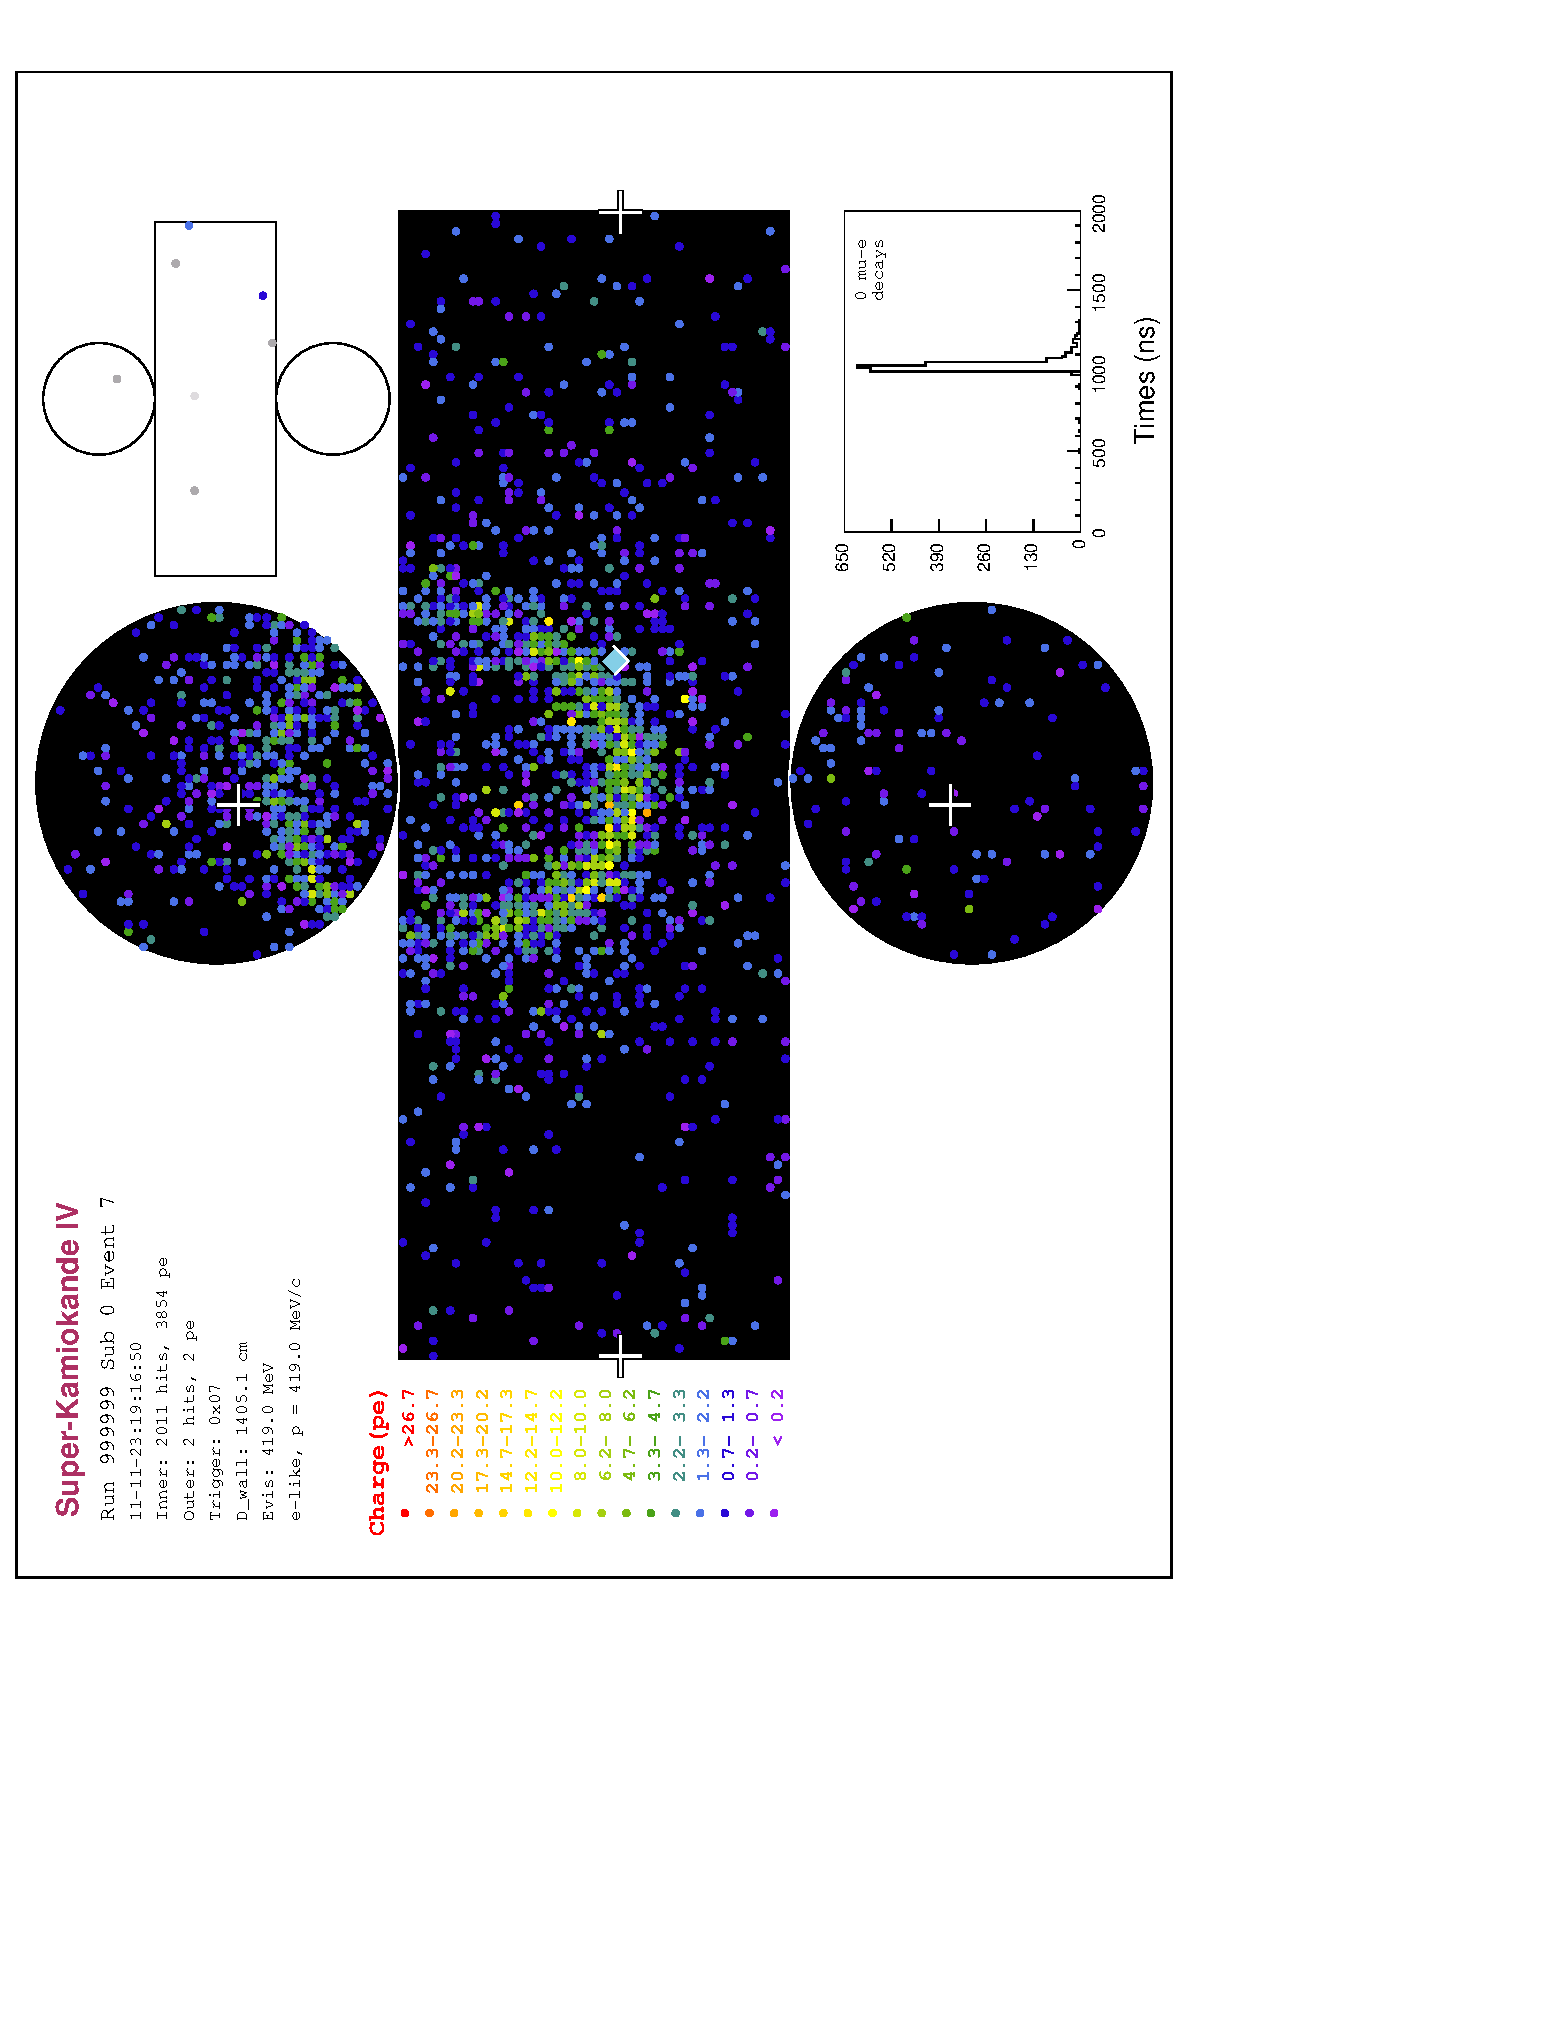
\includegraphics[width=\textwidth]{figures/t2k/sk-nue.eps}
        \caption{\(\nu_e\)}
        \label{subfig:sk-nue}
    \end{subfigure}
    \begin{subfigure}[b]{\dbfigwid\textwidth}
        \centering
        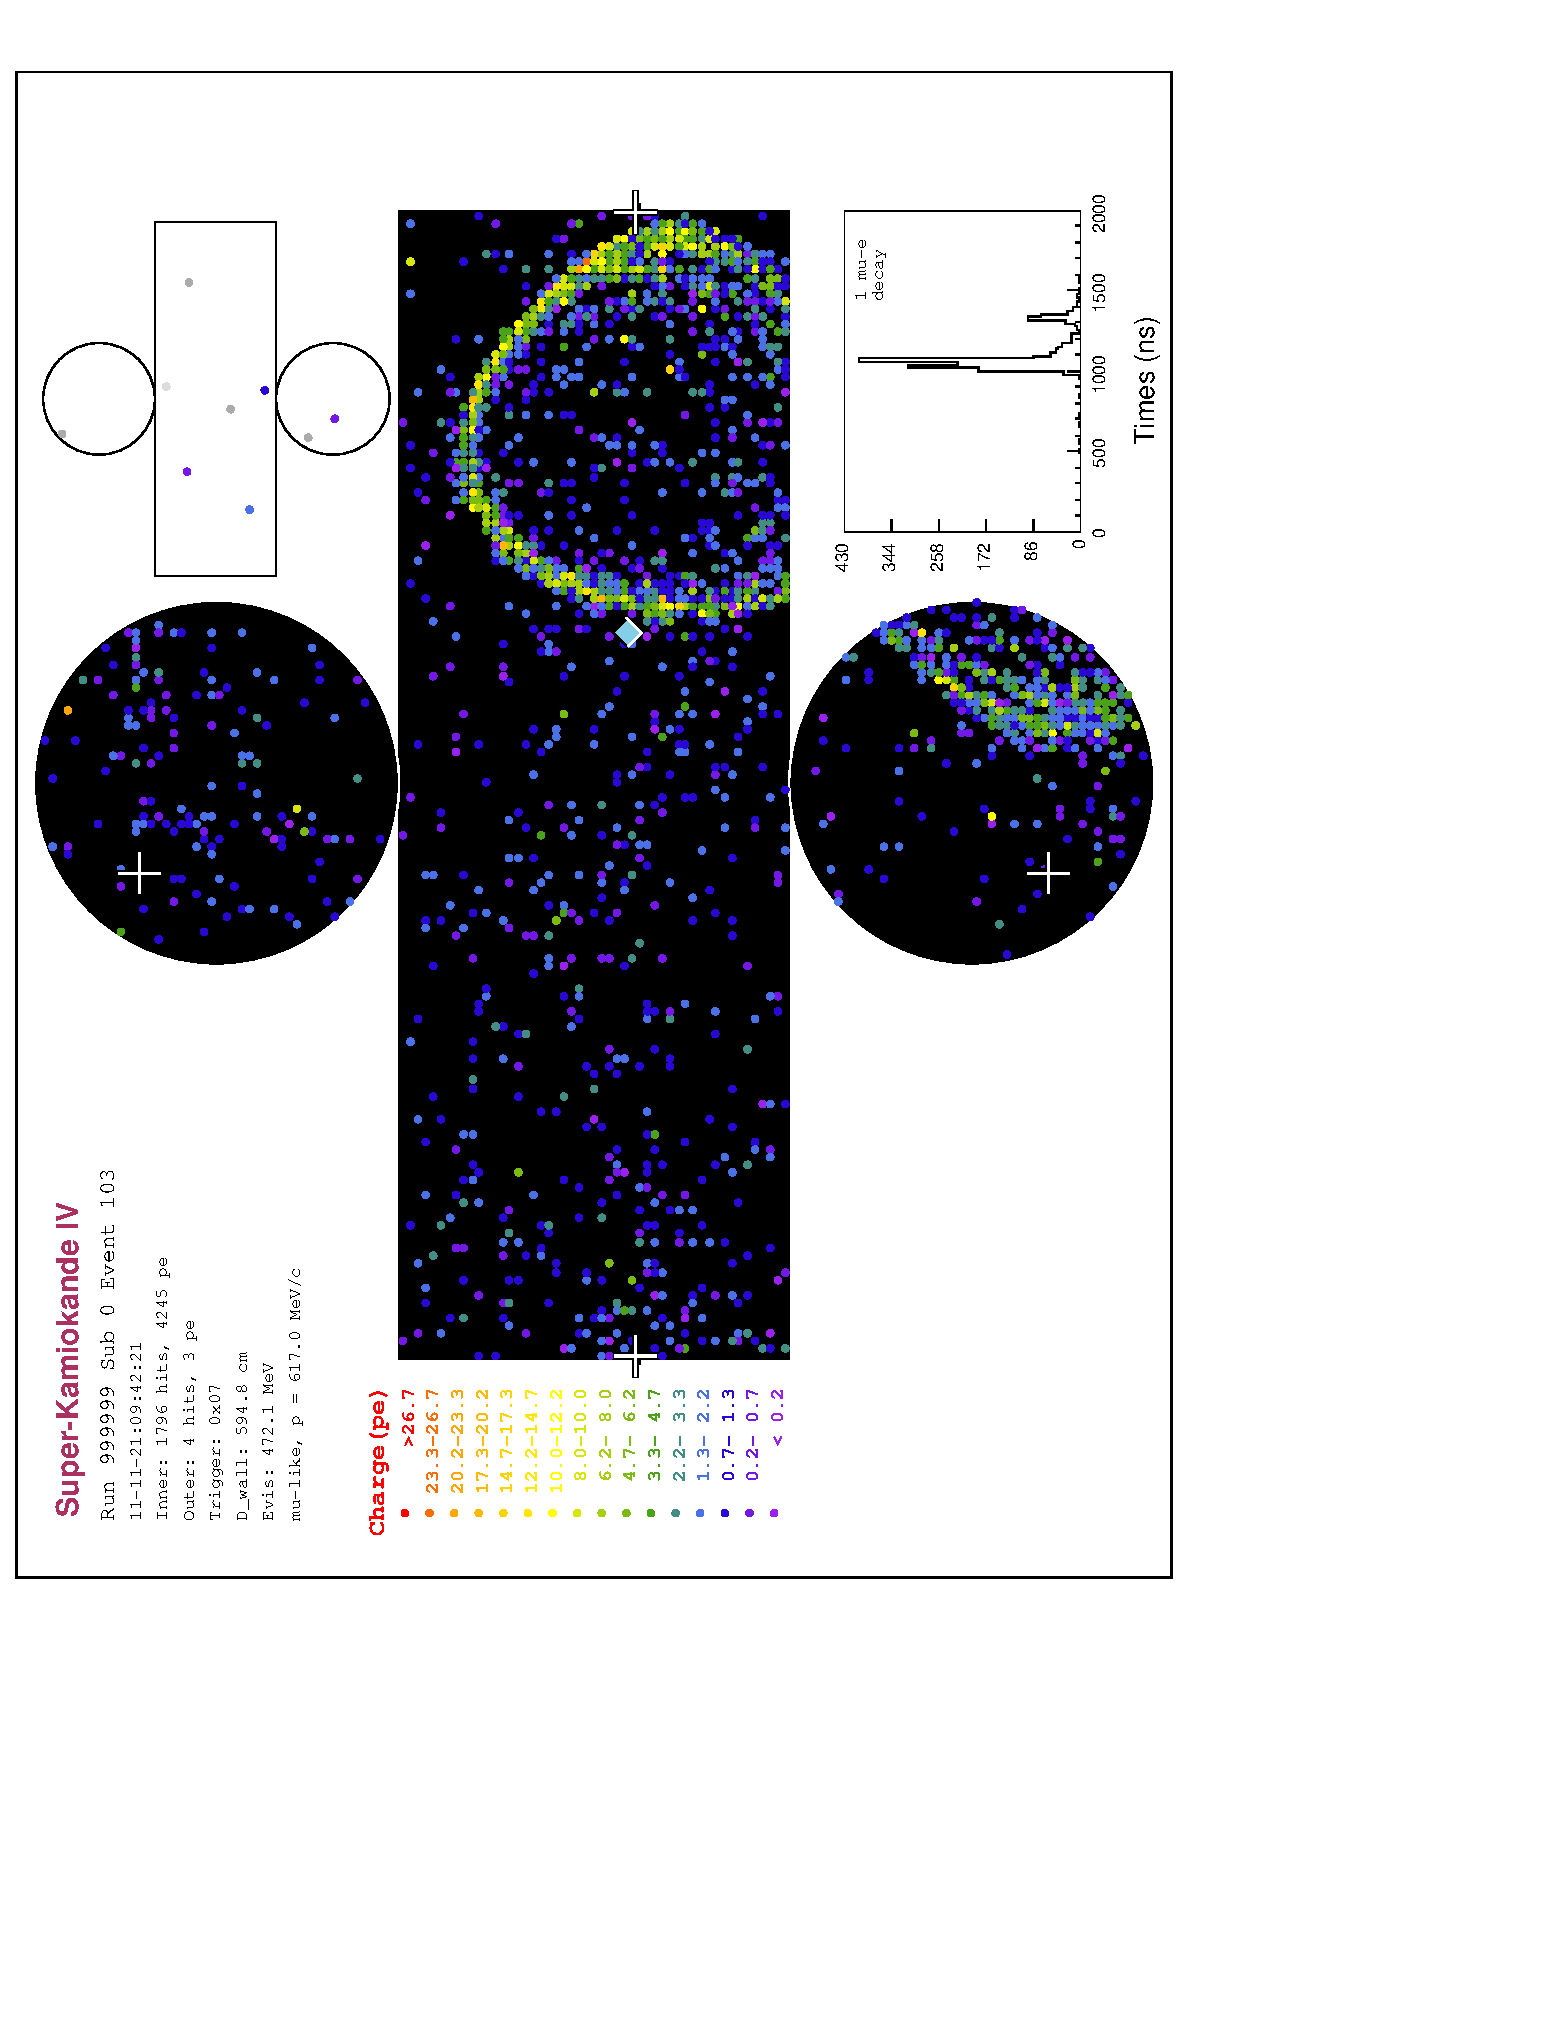
\includegraphics[width=\textwidth]{figures/t2k/sk-numu.eps}
        \caption{\(\nu_\mu\)}
        \label{subfig:sk-numu}
    \end{subfigure}
    \caption{SK event displays.}
    \label{fig:sk-e-mu}
\end{figure}

In contrast, the near detector, ND280, consists of multiple advanced subdetectors capable of detecting hadrons.
The classic ND280 is shown in Fig.~\ref{subfig:nd280-classic}.
The main detector assembly contains a \(\piz\)-detector (P0D), three vertical Time Projection Chambers (TPCs), and two Fine Grained Detectors (FGDs) sandwiched between the TPCs.
These detectors are surrounded by several electromagnetic calorimeters (ECALs)—the P0D ECAL, the Barrel ECAL, the Upstream ECAL, and the Downstream ECAL—which are in turn enclosed by the UA1 magnet composed of the solenoid coil and the yoke.

\begin{figure}
    \centering
    \begin{subfigure}[b]{\dbfigwid\textwidth}
        \centering
        \includegraphics[width=\textwidth]{figures/t2k/ND280-classic.eps}
        \caption{Classic}
        \label{subfig:nd280-classic}
    \end{subfigure}
    \begin{subfigure}[b]{\dbfigwid\textwidth}
        \centering
        \includegraphics[width=\textwidth]{figures/t2k/ND280-up.png}
        \caption{Upgrade}
        \label{subfig:nd280-up}
    \end{subfigure}
    \caption{ND280 detector diagram.}
    \label{fig:nd280-diagram}
\end{figure}

The neutrino beam traverses the P0D, TPCs, and FGDs.
The FGDs are made of scintillator bars with a cross section of \(1.0~\mathrm{cm} \times 1.0~\mathrm{cm}\).
Each layer of bars is oriented orthogonally to the previous layer.
As a particle passes through these layers, it excites photons in the scintillator, which are collected by wave-length shifting fibres running through each bar and ultimately read by end electronics.
Hence, track position information transverse to the neutrino beam is determined by the bar that recorded the signal, and the longitudinal information is given by the layer number at which the excitation occurs.

Before the upgrade, FGDs served as the active target for neutrino interactions.
However, the bar geometry yields a low acceptance for particles traveling at large angles to the beam direction (i.e.\ along the bar’s long axis), as they cross only a few bars and are thus difficult to reconstruct.
This mismatch in phase space between the near and far detector leads to extra uncertainties in oscillation analyses.
Additionally, having only a few signals along the particle trajectory degrades reconstruction resolution.
These drawbacks drove the ND280 upgrade.

In the upgraded ND280, the \(\piz\)-detector is replaced by a set of new subdetectors (Fig.~\ref{subfig:nd280-up}): the Time-of-Flight detector (TOF), two High-Angle TPCs (HATs), and the Super Fine Grained Detector (SFGD).
The TOF comprises six planes of scintillator bars, providing excellent sub-nanosecond timing resolution and effectively vetoing crossing particles, which enhances sample purity.
The HATs feature a redesigned field cage and new Micromegas, expanding the tracking volume and boosting resolution compared to the original vertical TPCs.
The SFGD, acting as the new active target, consists of about two million \(1\,\mathrm{cm}^3\) scintillator cubes.
Its finer granularity significantly improves acceptance for high-angle tracks and thus better matches the isotropic acceptance at the far detector.
Moreover, the enhanced tracking via improved energy deposition measurements lowers detection thresholds and boosts resolution, enabling novel reconstruction methods (e.g.\ trackless pion reconstruction) and creative variables (e.g.\ COM variables), to be introduced in the next chapter.
The upgrade was completed in April 2024, and the upgraded ND280 began taking data in June 2024.

\section{Software}
\label{sec:t2k-sw}
Much of this thesis focuses on improving reconstruction performance; thus, a broad overview of the reconstruction framework used for the ND280 upgrade is provided here to aid understanding.

Each scintillator cube in the SFGD holds an optical fibre, constituting an electronic signal channel.
As a particle passes through these cubes, scintillation photons are collected by readout boards on three orthogonal faces of the SFGD.
These signals are digitised after calibration, combining the three two-dimensional board outputs into a set of three-dimensional “Hits,” each corresponding to a cube position and carrying a measure of deposited charge.
The reconstruction software then groups these Hits into clusters or tracks via clustering and track-fitting algorithms.
Clusters are small collections of fewer than three Hits, while tracks contain many more.
Additionally, due to imperfect optical isolation between cubes, some photons may leak into adjacent cubes that the particle did not actually traverse.
Hence, the reconstruction merges nearby Hits into “Nodes,” more accurately reflecting the particle’s path.
Energy deposition at each Node is then estimated from the included Hits and smoothed according to the physical expectation of continuous energy loss along the track.
Next, a Boosted Decision Tree (BDT) trained on Particle Gun (PGUN) simulations uses these smoothed energies and other measured quantities to perform particle identification and momentum estimation.
